\subsection{The \NHD\ detector}
\label{sec.hd}

\begin{figure}[htbp!]
\centering
    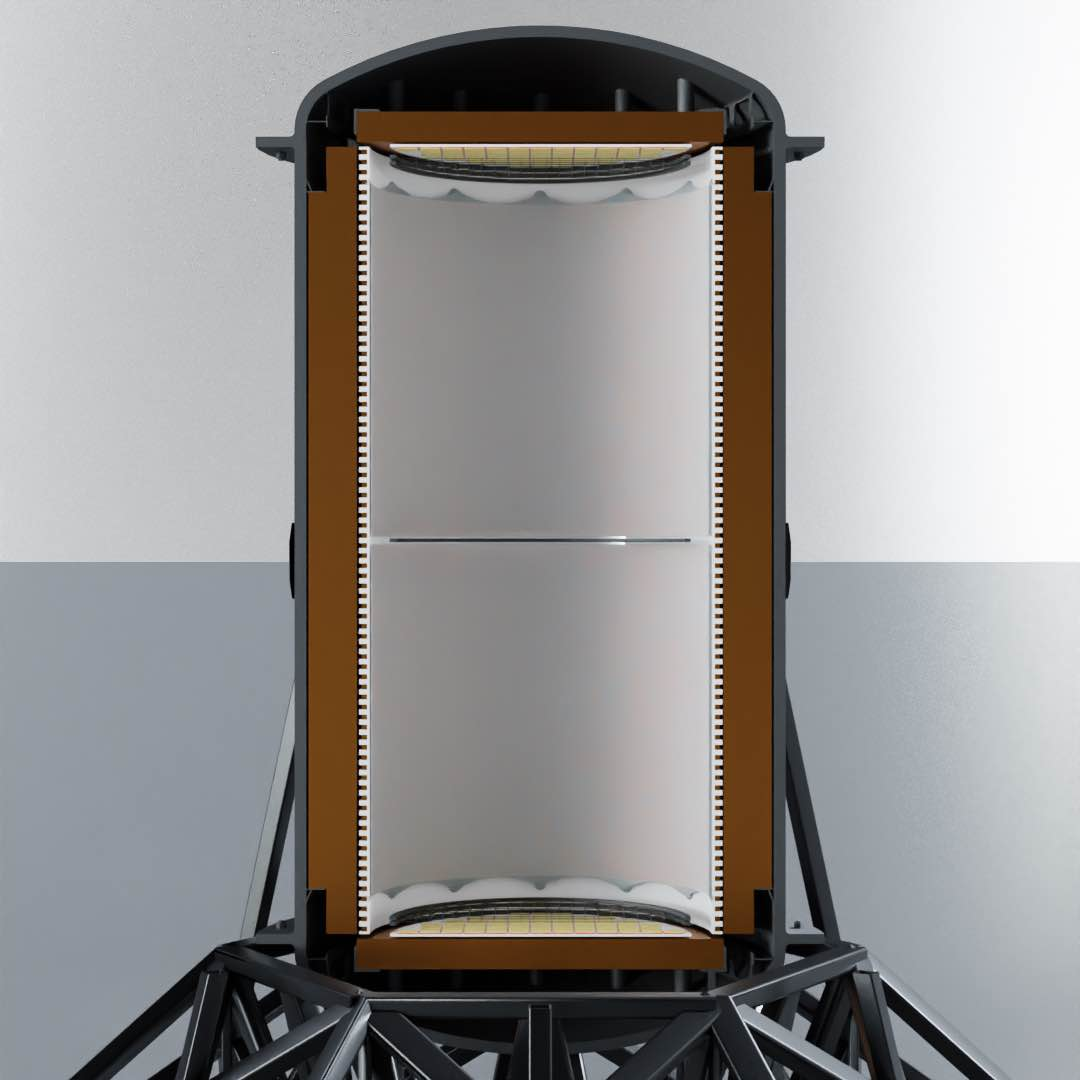
\includegraphics[width=0.42\linewidth]{img2/cut_detector.jpg}
    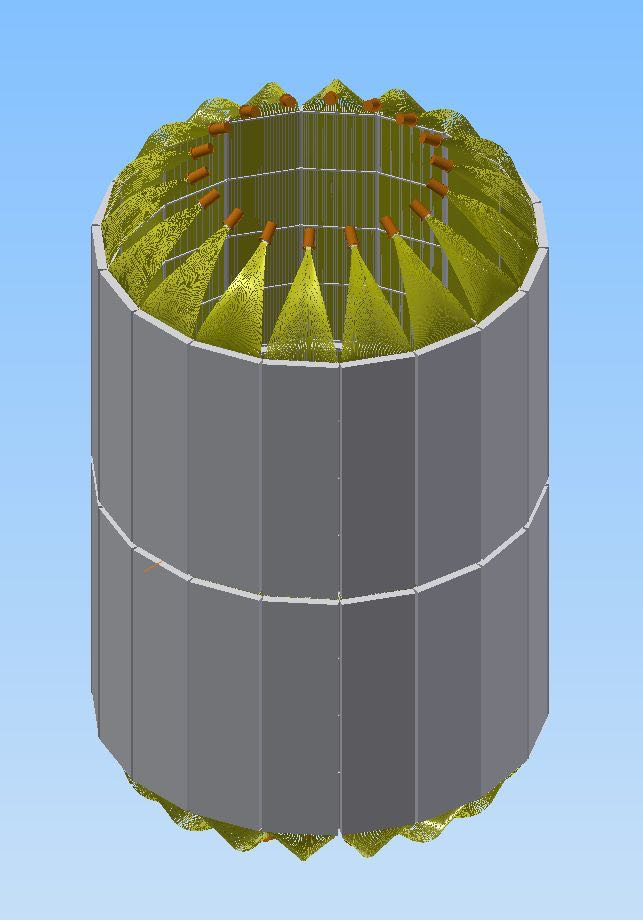
\includegraphics[width=0.30\textwidth]{img2/Fiber23D.jpg}
    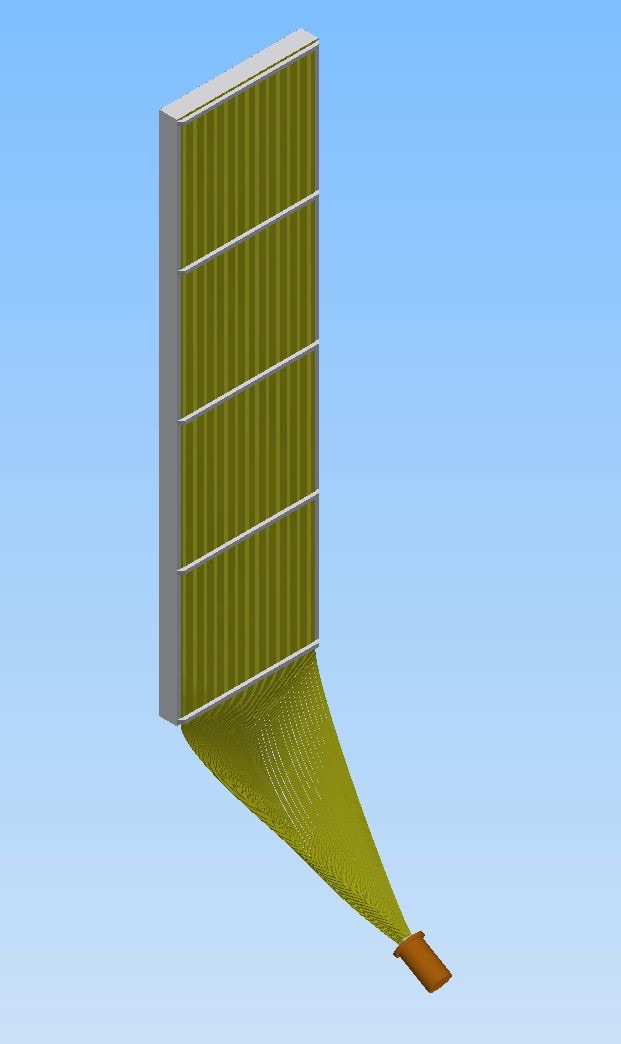
\includegraphics[width=0.26\textwidth]{img2/FiberPanel.jpg}
    %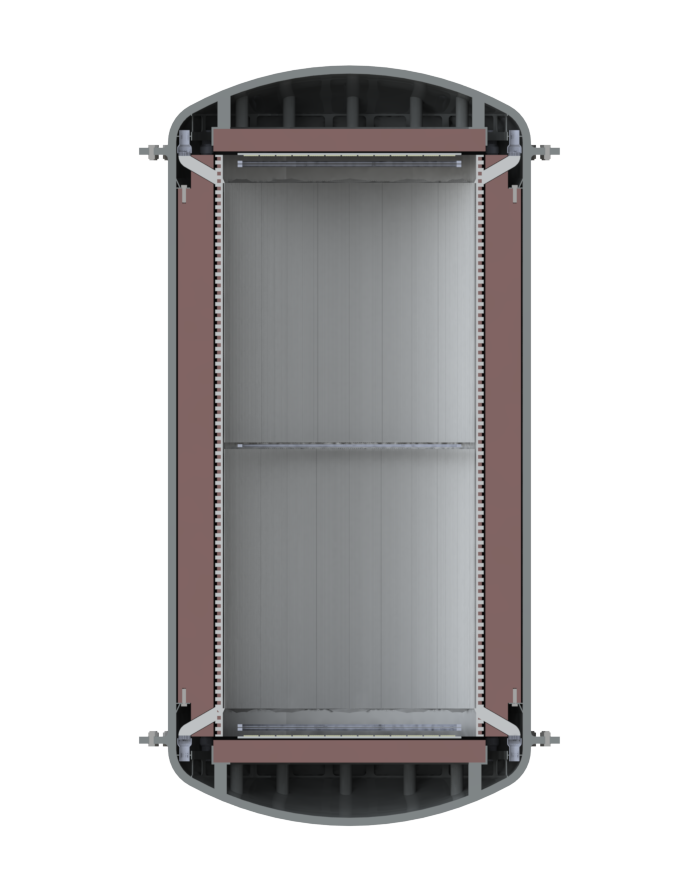
\includegraphics[width=0.42\linewidth]{img/Half_5.png}
     \caption{\small Left: image of the \NHD\ detector in its vertical orientation. Middle: conceptual drawing of the BFD. 
     Right: conceptual drawing of  a fibre panel.}
     \label{fig.NHD}
\end{figure}

%\begin{figure}
%  \begin{center}
%    %\includegraphics[width=0.31\textwidth]{img/Fiber13D.png}
%    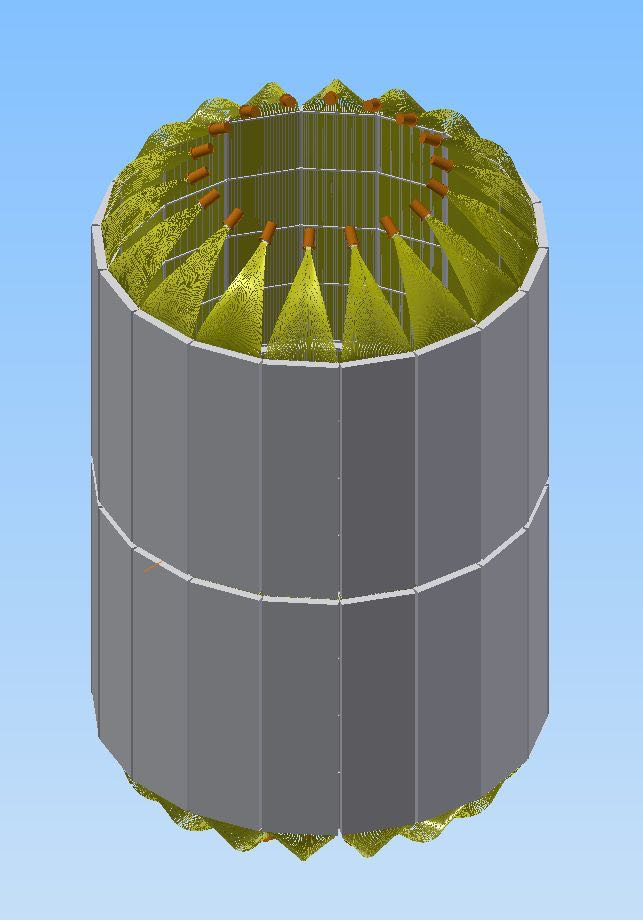
\includegraphics[width=0.31\textwidth]{img2/Fiber23D.jpg}
%    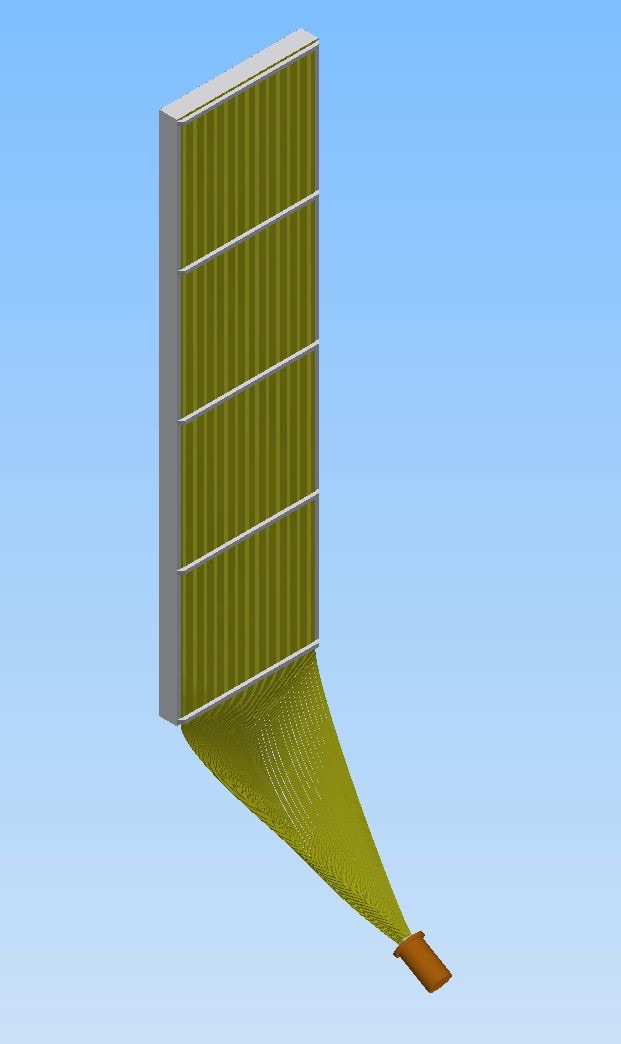
\includegraphics[width=0.25\textwidth]{img2/FiberPanel.jpg}
%    \caption{Conceptual design of the BFD (left), and of a fibre panel (right).} 
%    \label{fig.BFD}
%  \end{center}
%\end{figure}

\begin{figure}
  \begin{center}
      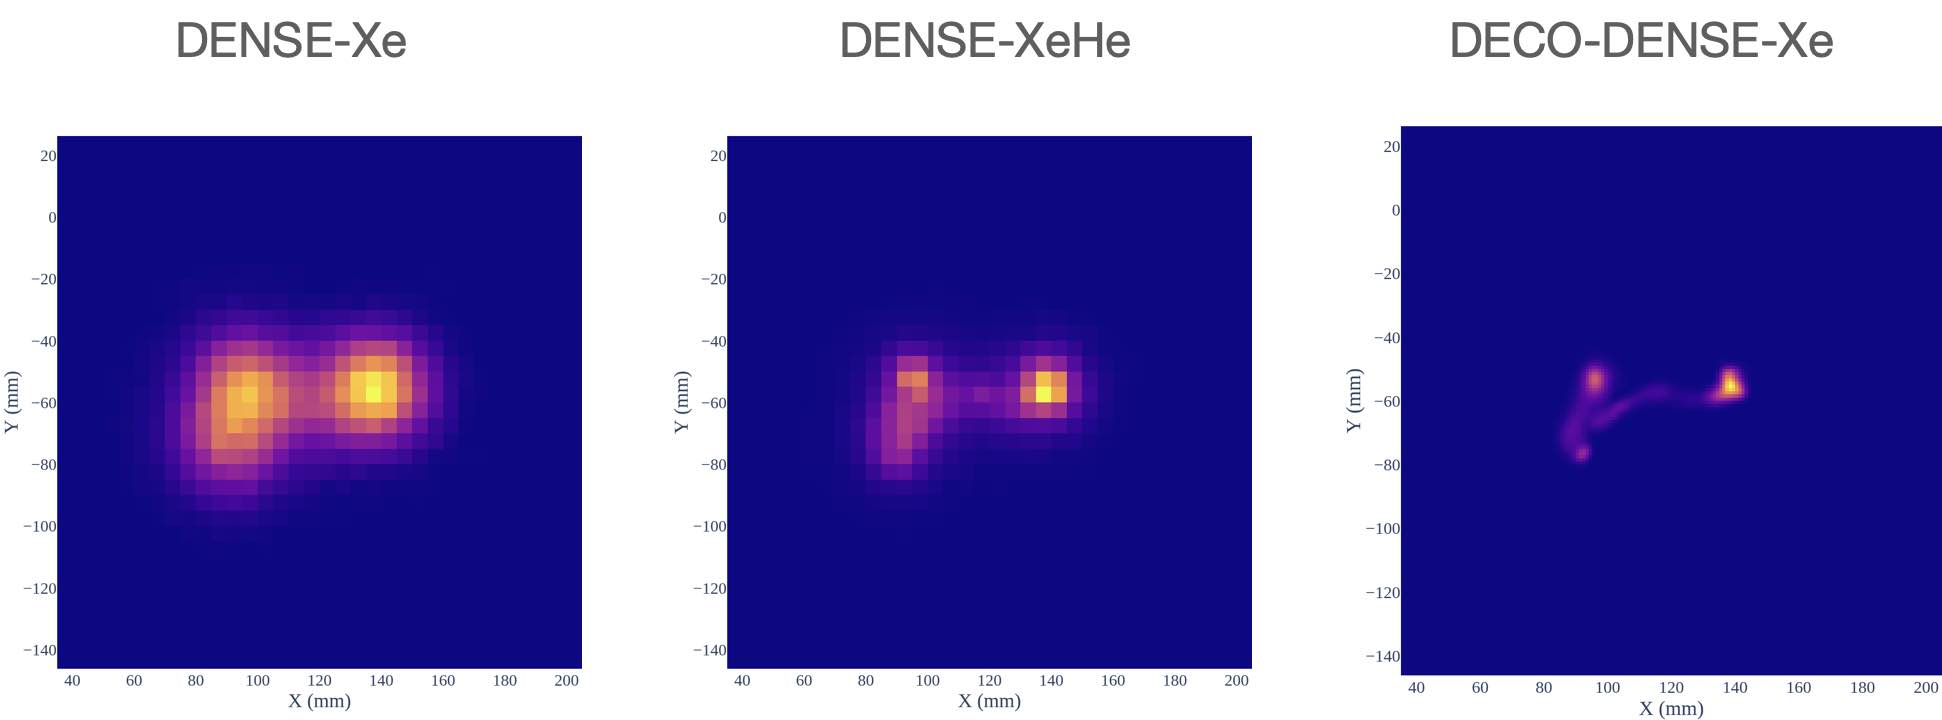
\includegraphics[width=0.91\textwidth]{img2/tracks.jpg}
    \caption{Impact on track reconstruction of reduced diffusion and fine grain tracking planes (DSPs). The let panel shows the signature of the two electrons emitted in a \bb\ decay, when reconstructed with a dense silicon plane. Notice the separation between the two ``blobs'', each one defining the end-point of one electron. The middle panel shows the same reconstruction when using a low diffusion mixture with 15\% Helium. The right panel shows the final double electron, reconstructed after our sophisticated deconvolution technique (see \cite{NEXT:2020jmz}).} 
    \label{fig.DSP}
  \end{center}
\end{figure}


 The HPXe technology benefits from the economy of scale inherent to homogeneous experiments in which the \bbonu\ source and the detector are the same. The necessary factor of 10 increase in fiducial mass is obtained by increasing the detector linear dimensions (parallel and perpendicular to the TPC drift direction) by slightly more than a factor of 2 compared to \NEXT. At the same time, the background rate (after cuts) must be kept in the ``quasi-zero'' regime of less than one event per year in the ROI. This requires a detector with improved radiopurity at the ton-scale. This is achieved by the combination of: {\bf i)} a reduced background budget, achieved, in particular, by eliminating the leading source of background (the PMTs of the EP, which is replaced by a low-background system, the barrel fiber detector, BFD) and further reduce other background sources (thinner kapton boards, titanium frames for the grids and ultra-low radioactivity resistors);  {\bf ii)} improvement of the energy resolution from 1\% to 0.5--0.7\% FWHM at \Qbb, possible thanks to the better  performance of BFD which collects more light than \Next\ EP and is less affected by geometrical corrections; and {\bf iii)} improvement of the rejection power of the topological signature, by reducing the diffusion through the use of low-diffusion Xe-He mixtures. The resulting apparatus will have ``higher definition'' of the signal, w.r.t. previous NEXT apparatus, thus the label HD (``high definition''). 
 
 \indent
 
The \NHD\ concept is schematically rendered in the left panel of figure \ref{fig.NHD}. %shows a conceptual rendering of the \NHD\ detector.
The major change in the design with respect to the current apparatus is the transformation to a symmetric device featuring two twin back-to-back TPCs, each  with its own EL region and connected by a central cathode. In a symmetric detector, one doubles the active region for the same cathode voltage compared to its asymmetric counterpart.  Based on geometrical considerations the required high voltage for \NHD\ will be only $\sim$ 30\% larger than that needed for NEXT-100. A symmetric detector with 2$\times$\XHDL drift and \XHDD\ diameter will be able to hold \XHDM\ at 15 bar. Another relevant modification with respect to NEXT-100 is the vertical detector orientation, chosen in order to simplify the assembly of the different parts of the system, in particular the heavy (about \XHDS) inner copper shield. 

\indent

The second major change ---dictated by both the symmetric detector design and the need to reduce the background budget--- is the substitution of the energy plane (made of PMTs viewing the active volume) by an alternate energy measurement solution.  An attractive solution is a barrel detector made of wavelength-shifting optical fibres. The fibres, coated with tetraphenyl-butadiene (TPB) shift first the impinging VUV photons to violet photons (with an average wavelength circa \SI{420}{\nm}). Those photons are absorbed by the fibers which re-emit green light (circa  \SI{530}{\nm}). Green photons propagating by total internal reflection inside the double-clad fibres reach the fibres ends, which are grouped in bundles and read out by either PMTs or SiPMs. Our Monte Carlo studies show that the light collection of this Barrel Fibre Detector (BFD) is at least 50\% larger than that of a conventional NEXT energy plane. This, together with the expected soft geometrical corrections (which, to first order, should follow a smooth radial dependence) would imply a corresponding improvement in the detector energy resolution. The BFD will also measure \sone, providing the start-of-the-event.  The middle and right panels of figure \ref{fig.NHD} show conceptual drawings. 

\indent

Last but not least, the possibility to reduce diffusion and thus improve the rejection power of the topological signature calls for a fine granularity tracking system. Dense SiPM planes (DSPs), with a pitch of the order of \SI{7}{\mm}) will allow a better measurement of the track trajectories. The impact of reduced diffusion and fine granularity is illustrated in figure  \ref{fig.DSP}. 
%Notice that the reconstruction using fine grain pixels provided by the DSPs, and helium-xenon mixtures, together with the sophisticated deconvolution developed by NEXT \cite{NEXT:2020jmz} results in tracks very similar to those obtained by pure Monte Carlo simulation, showing that one can maximally exploit the electron identification. 

%The DSPs also provide two independent measurements of the energy of the event, one in the plane where the EL is produced and another in the opposite plane, the two measurements being affected by different geometrical corrections. The two DSP energy measurements are also statistically independent of the energy measurement provided by the BFD. According to our calculations, this redundancy may provide an improved energy resolution, in the range 0.5--0.7\% FWHM at \Qbb. 

\indent

Finally, the shielding of \NHD\ will be different from that of \Next. The need to suppress drastically cosmogenic backgrounds at the LSC depth (which requires a very effective veto against muon-induced neutrons and energetic gamma-rays) leads to replacing the lead structure (``lead castle'') used by \Next\ by an instrumented water tank (WT). In addition, the detector will have (like \NEW\ and \Next\ an inner copper shield to protect the TPC volume from backgrounds emanating from the vessel). 


%%%%%%%%%%%%%%%%%%%%%%%%%%%%%%%%%%%%%%%%%%%%%%%%%%%%%%%%%%%%
\subsubsection{Sensitivity of \NHD}
\label{sec:BackgroundsAtTheTonneScale}
%%%

The sensitivity of \NHD\ has been extensively discussed in a recent publication \cite{NEXT:2020amj}. Here we summarise the main results. 
Our background model and event selection algorithms, described below, have been checked against the data collected by \NEW\ \cite{Novella:2019cne} and will be further validated to higher precision with the data acquired  by \Next. 

\indent

{\bf $\bullet$~ Backgrounds of radiogenic origin}

\indent
High-energy gamma radiation from long-lived radioactive contaminants present in detector materials and surroundings is an important background in NEXT. Particularly troublesome are two of the gamma-ray lines emitted following the decays of \Tl{208} and \Bi{214}, part of the thorium and uranium series, respectively. The gamma-ray line from \Tl{208} (2614.5~keV, 99.75\% intensity \cite{nudat}) is well above $\Qbb=\SI{2457.8}{\kilo\eV}$, the $Q$ value of \Xe{136}, but single-electron tracks from its photopeak can lose energy via bremsstrahlung and fall in the region of interest. Likewise, gammas that interact via successive Compton scatters in proximity may be reconstructed in some cases as a single track with energy close to \Qbb. The gamma-ray line from \Bi{214} (2447.7~keV, 1.55\% intensity \cite{nudat}) lies just below \Qbb, and thus its photopeak can overlap with the \bbonu\ peak due to the finite energy resolution of the detector.

\indent

Gamma radiation emanating from laboratory walls and external support structures is unlikely to reach the inner detector through the water shielding (3~m of water attenuate this gamma flux by more than 6 orders of magnitude). For this reason, we focus on sources close to the active volume of the detector, particularly those with large mass, such as the inner copper shield. These backgrounds can be mitigated and understood by careful radio assay of all materials used in the construction of the detector. The NEXT Collaboration has undertaken extensive campaigns for the characterisation of all materials used for the \NEW\ and NEXT-100 detectors \cite{Alvarez:2012as, Cebrian:2017jzb}, primarily employing gamma-ray spectroscopy with high-purity germanium detectors and inductively coupled plasma mass spectrometry (ICPMS). An even more extensive and stringent campaign will be even more important for the material selection of \NHD, under the coordination of the LSC.  


%%%%%%%%%%
%\begin{table}[tb]
%\centering
%\begin{tabular}{l l l c c c}
%\toprule
%Material & Detector system & Method & \multicolumn{2}{c}{Activity ($\mathrm{\mu Bq / kg}$)} & Reference \\
%         &                 &        & \Th{232} & \U{238} & \\
%\midrule
%Copper & Inner shield   & ICPMS            & $1.22\pm0.04$   & $1.28\pm0.09$ & \cite{NEXT:2020amj} \\
%PTFE   & TPC field cage & NAA              & $0.103\pm0.012$ & $<5$          & \cite{Abgrall:2016cct} \\
%Kapton & Readout planes & ICPMS            & $81\pm15$       & $110\pm50$    & \cite{Arnquist:2019fkc} \\
%\bottomrule 
%\end{tabular}
%\caption{Specific activities of \Th{232} and \U{238} (parents of \Tl{208} and \Bi{214}, respectively) assumed in the background model of NEXT-HD for the most relevant materials used in the detector.}
%\label{tab:RadioactivityMaterials}
%\end{table}
%%%%%%%%%%

\indent

The material that dominates the budget is copper, given the large mass (nearly 40~tons) used for the inner shield. 
%Our best activity measurement (C11000 copper supplied by Lugand Aciers, radio assayed at PNNL using ICPMS) is comparable to values reported elsewhere \cite{Kharusi:2018eqi}. 
After copper, PTFE and Kapton, two synthetic polymers, are the main contributors to the radioactivity budget of \NHD. PTFE (about \SI{500}{kg}) represents a significant fraction of the mass of the TPC field cage. Backgrounds from the pressure vessel as well as any additional infrastructure outside the detector are efficiently mitigated by the inner copper shielding. They are estimated to contribute at or below the 5\% level to the full radioactive budget. 
%Here, we use activity measurements reported in the literature \cite{Abgrall:2016cct}. In the case of Kapton, used as substrate for the SiPM support boards (each one is \SI{8.4}{g} and covers \SI{121}{cm^2}), we use recently-published measurements \cite{Arnquist:2019fkc}. 


%This number is informed by experience from \NEW\ and NEXT-100, where present upper limits sit at approximately 5--10\% of the total activity budget \cite{Martin-Albo:2015rhw, Novella:2019cne}. Any additional external sources can be effectively mitigated by increasing the thickness of inner copper shielding without significant detriment to the total activity.

\indent

Radon is another potential source of radioactive background, since it can diffuse from detector materials or the gas system and enter the active region. Only two radon isotopes, \Rn{220} and \Rn{222}, from the thorium and uranium series, respectively, are found in significant amounts. Their production rates are similar, but the longer half-life of the latter (3.8~days versus the 56~seconds of \Rn{220} \cite{nudat}) makes it much more likely to become a background. Radon-222 undergoes two alpha decays to produce \Bi{214}, and previous NEXT measurements show that these positively-charged daughters usually plate out onto the cathode \cite{Novella:2018ewv}. The subsequent \Bi{214} decays on the cathode are rejected with high efficiency (through fiducial cuts) by the detection of the emitted beta electrons and coincident decays of \Po{214}. Rejection efficiency should only increase in a symmetric design, since the cathode would be surrounded by fully instrumented volumes. For the present study, we consider the internal radon backgrounds at a similar rate as that of the present generation of NEXT detectors~\cite{Novella:2018ewv}, a conservative assumption, given the improvements in radiopurity expected in \NHD. Additional contributions from airborne radon backgrounds from outside the vessel are expected to be negligible due to the surrounding water.

%%%%%%%%%%%%%%%%%%%%%%%%%%%%%%%%%%%%%%%%%%%%%%%%%%%%%%%%%%%%
{\bf $\bullet$~ Backgrounds of cosmogenic origin}
\label{sec:muons}
%%%
Cosmogenic backgrounds in NEXT derive from neutron capture on detector materials, especially on copper isotopes and \Xe{136}. The main source of neutrons that induce these potential backgrounds are atmospheric muons with energies up to a few TeV that reach the laboratory through the rock overburden. 
%Neutron capture produces two types of potential background: prompt activity from gamma radiation post-capture, and the creation of long-lived nuclei with decays that can result in events at energies close to \Qbb. The former is dominated in NEXT by contributions from the capture of neutrons on the two main copper isotopes via the reactions $^{63,65}\text{Cu}(n, \gamma)^{64,66}\text{Cu}$ \cite{nudat}, but there are also contributions from captures on plastics and on the steel pressure vessel. The cascade photons from all of these various reactions have energies up to tens of MeV. As the interactions in the gas occur within a few ms of the passage of a muon, these events can be rejected without significant reduction to detector live-time, introducing a veto of \SI{2}{\milli\second} after the tagging of a muon in the water tank or the TPC. Any remaining events contribute at a negligible level.

\indent

%Non-prompt backgrounds derive from the production of long-lived isotopes that later decay with $Q$ values above \Qbb. 
The dominant contribution to this background comes from the beta-emitter \Xe{137}, produced by single-neutron capture on \Xe{136}. Xenon-137 decays with a half-life of \SI{3.8}{minutes} and a $Q$ value of \SI{4.17}{\mega\eV} \cite{nudat}. This background is difficult to veto by time coincidence with a detected muon due to the excessive dead-time that it would generate. 


%%%%%%%%%%%%%%%%%%%%%%%%%%%%%%%%%%%%%%%%%%%%%%%%%%%%%%%%%%%%
\indent

{\bf $\bullet$~ Signal efficiency and background rejection}
\label{sec:SimulationAndAnalysis}

\indent

%%%

%%%%%%%%%%
\begin{figure}
\centering
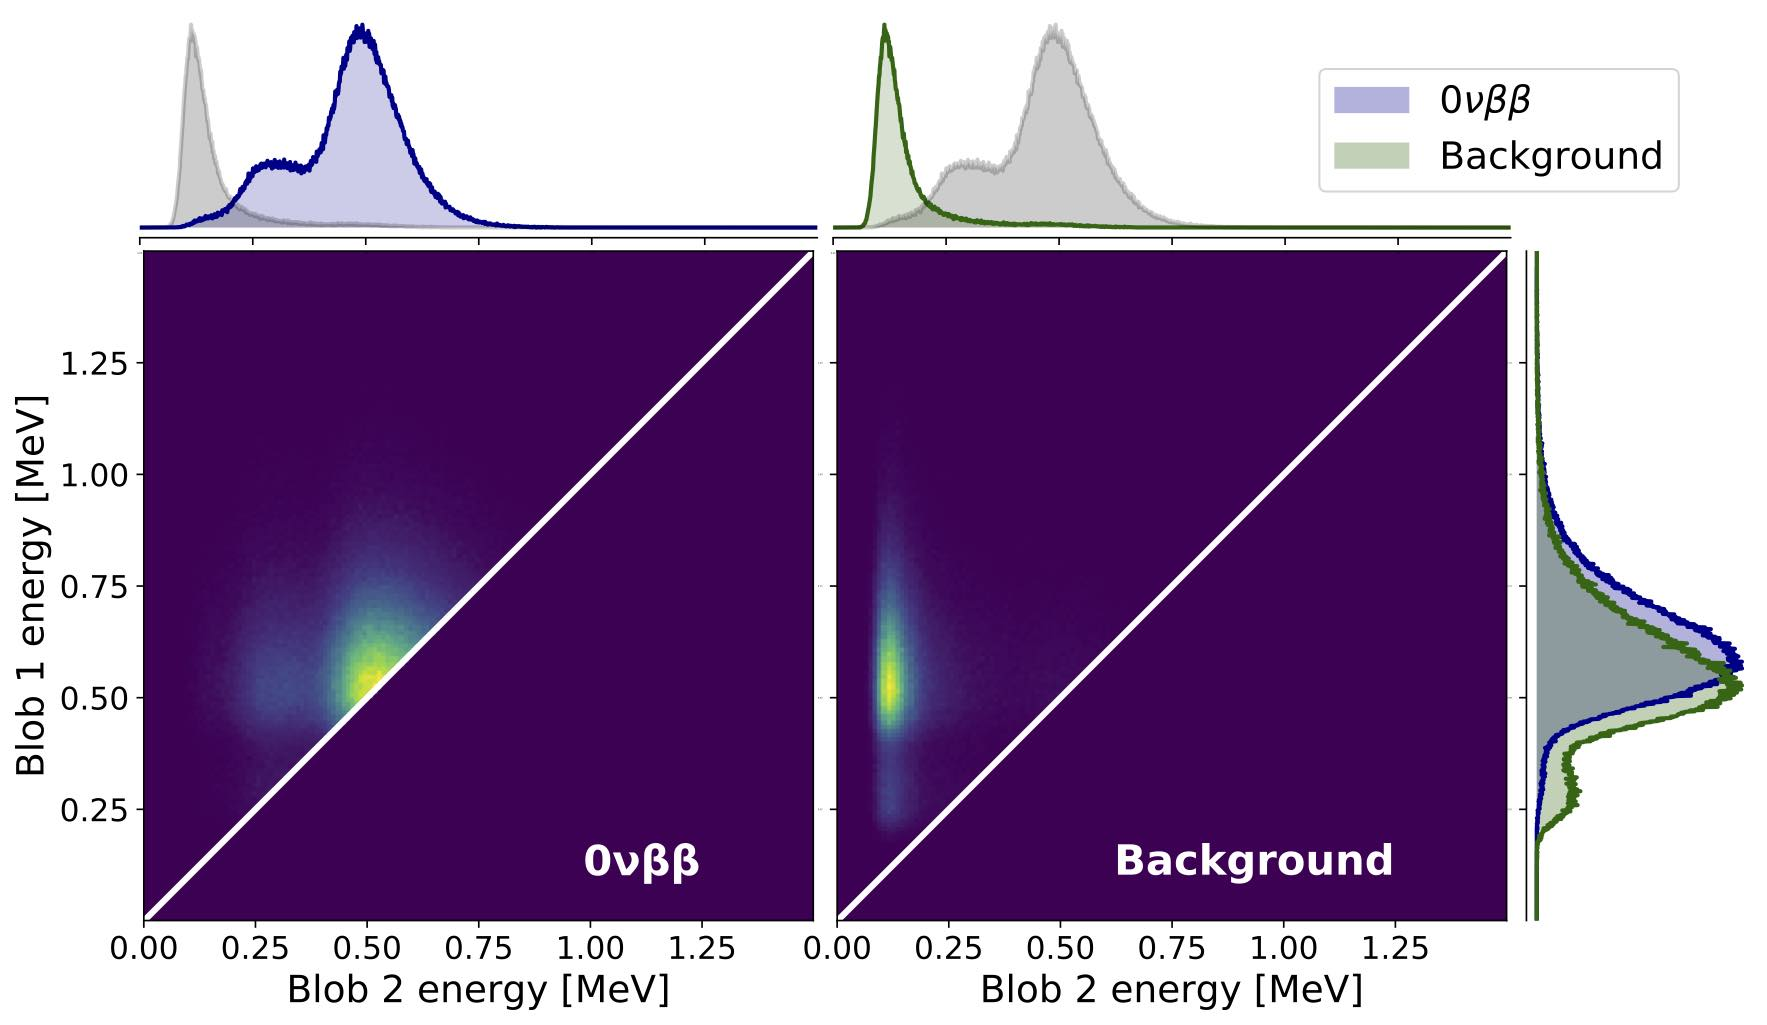
\includegraphics[width=0.55\textwidth]{img2/BlobComparison.jpg}
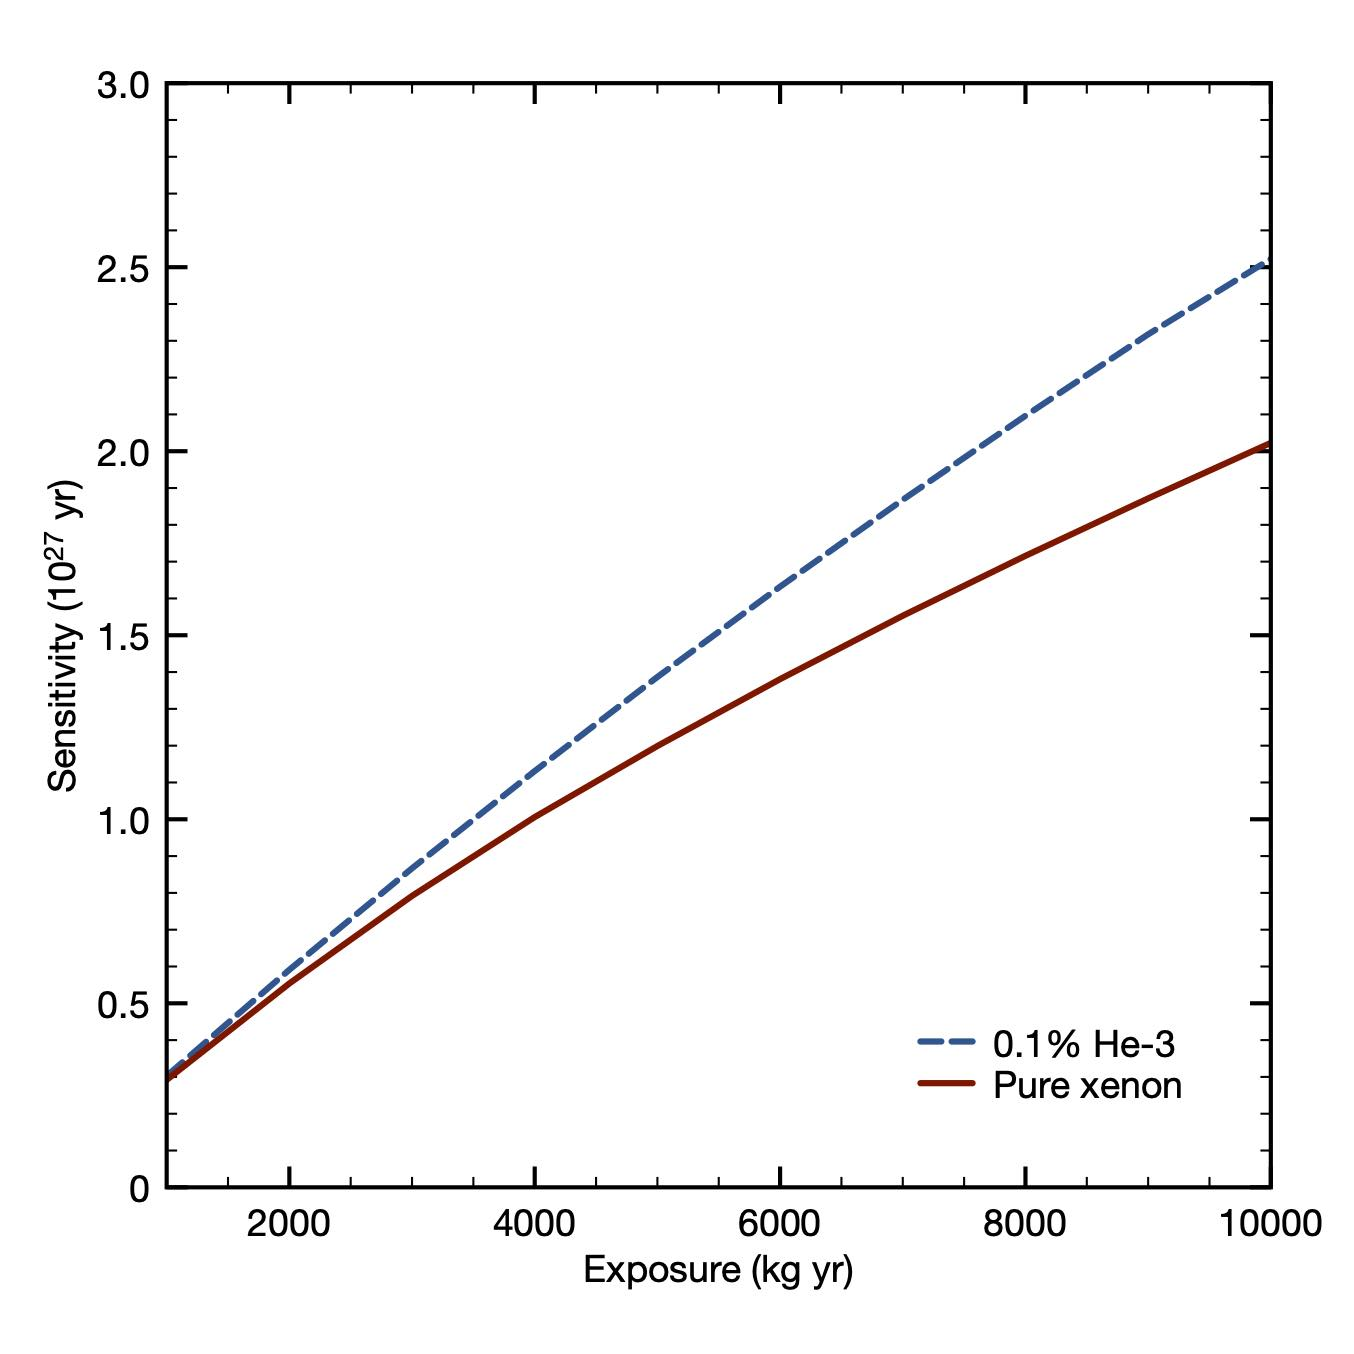
\includegraphics[width=0.40\textwidth]{img2/sensitivity_nexthd_lsc.jpg}
\caption{Left: blob energies of signal and background events. The blobs are defined such that \emph{blob 1} always has higher energy. Right: sensitivity of \NHD.}
\label{fig:blobs}
\end{figure}
%%%%%%%%%%

We evaluated the signal efficiency and background rejection of \NHD\ following the methodology described in \cite{Martin-Albo:2015rhw, NEXT:2020amj}. Signal events in NEXT have a distinctive energy-deposition pattern: a continuous track with large energy deposits (or \emph{blobs}) at both ends. Background events, in contrast, are generated mostly by single electrons, thus having only one end-of-track blob. The separation between signal and background events is illustrated in the left panel of figure~\ref{fig:blobs}, which shows the blob energy distributions for all signal and background events generated for the study. The figure of merit indicates a threshold of \SI{400}{\kilo\eV} as the optimal for the lower blob energy.

\indent

The main components of the radioactive budget before and after selection cuts are presented in figure \ref{fig:ActivityComp}. The contribution of the cosmogenically-induced \Xe{137} is 2.5 times as large as the radiogenic background at the depth of LSC (2500~m.w.e.). Nevertheless, the cosmogenic background could be mitigated with the addition of \He{3} to the xenon as a means to moderate and capture neutrons, reducing the number of activations in the detector volume. A reduction in the number \Xe{137} of over 1 order of magnitude could be achieved with as little as 0.1\% by mass of \He{3} doping \cite{rogers2020mitigation}. The possibility to procure \He{3} for the NEXT experiment is being explored by the US groups in the collaboration. 

%%%%%%%%%%
\begin{figure}[tb]
\centering
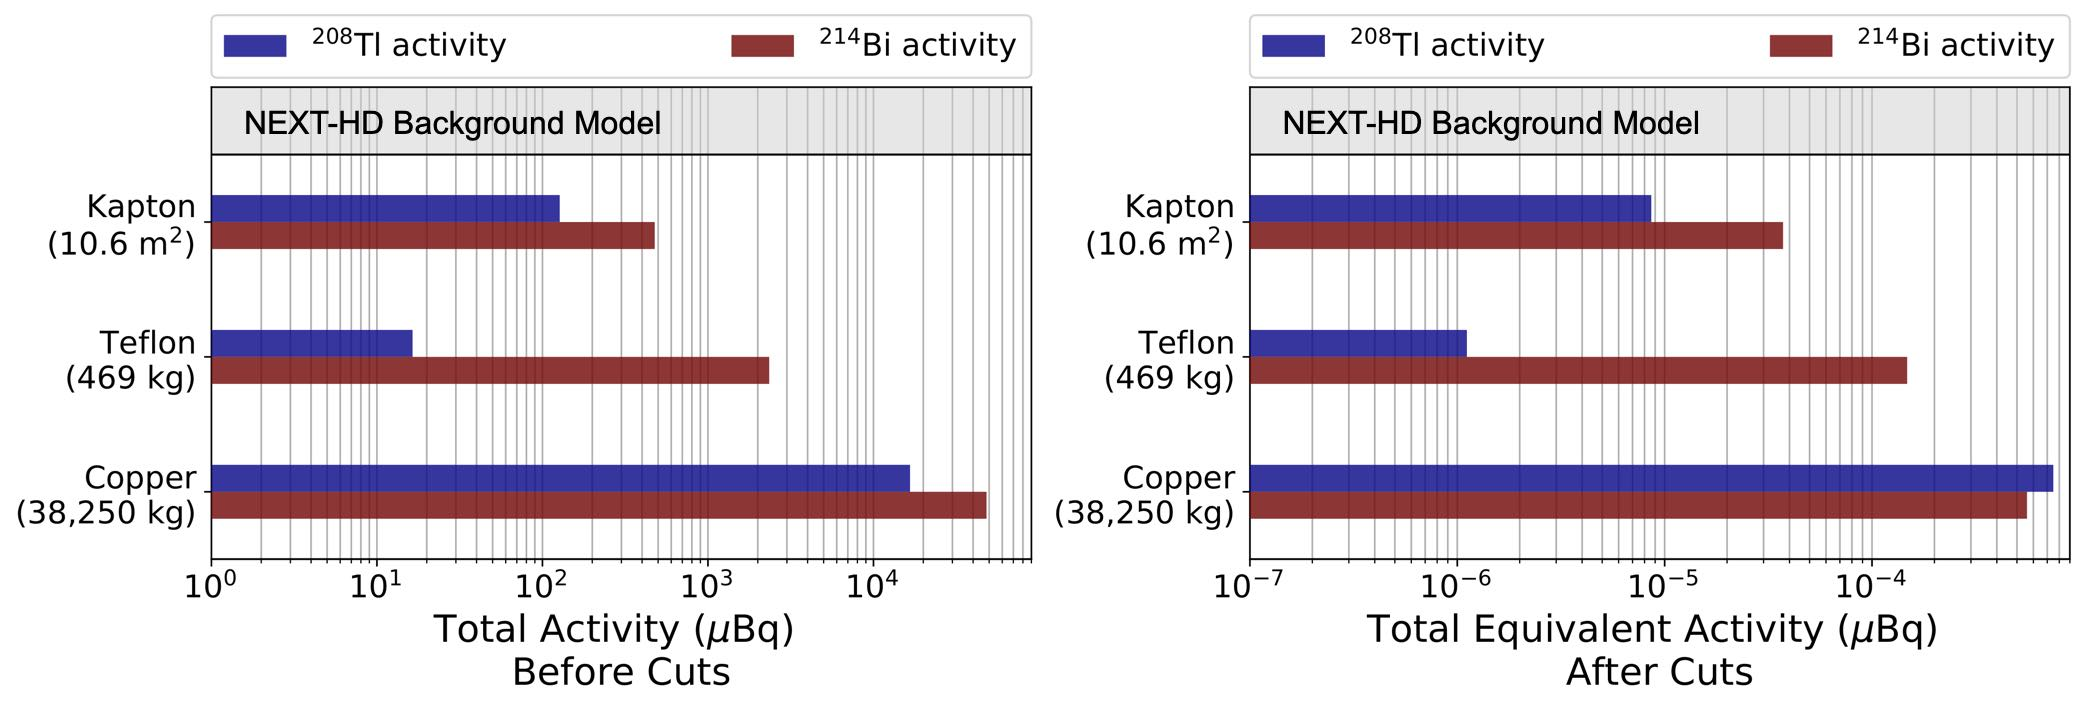
\includegraphics[width=0.90\textwidth]{img2/RadioactiveBudget2.jpg}
\caption{Left: Total background activity before cuts for the dominant sources in the \NHD\ radioactivity budget. Right: Activity remaining after selection cuts.}
\label{fig:ActivityComp}
\end{figure}
%%%%%%%%%%

%%%%%%%%%%
%\begin{table}
%\centering
%\begin{tabular}{lccS[table-format=2.2e-1]}
%\toprule
%Det.\ system & \multicolumn{2}{c}{Acceptance [$10^{-8}$]} & {Background index} \\
% & \Tl{208} & \Bi{214} & {[$\mathrm{ton^{-1}~yr^{-1}~ROI^{-1}}$]} \\
%\midrule
%Field cage        & 6.80(90) & 6.30(80) &  4.25e-3 \\ \addlinespace
%Readout planes    & 6.80(90) & 7.80(80) &  1.36e-3 \\ \addlinespace
%Inner shielding   & 4.50(70) & 1.20(70) & 37.23e-3 \\ \addlinespace
%Radon (cathode)   & ---      & 0.10(10) &  2.72e-3 \\ 
%\bottomrule
%\end{tabular}
%\caption{Acceptance factor (i.e., the probability of accepting a background event as signal) and resulting background indexes per unit of mass of \Xe{136} for the natural-radioactivity background sources considered in the background model of \NHD.}
%\label{tab:radiogenics}
%\end{table}
%%%%%%%%%%

%%%%%%%%%%
%\begin{table}
%\centering
%\begin{tabular}{lcS[table-format=2.2e-1]}
%\toprule
%Source gas & Acceptance  & {Background index} \\
% & [$10^{-5}$] & {[$\mathrm{ton^{-1}~yr^{-1}~ROI^{-1}}$]} \\
%\midrule
%Pure xenon & \multirow{2}{*}{5.68(17)} &  113.49e-3\\ \addlinespace
%0.1\% \He{3} doping &  & 11.78e-3 \\ 
%\bottomrule
%\end{tabular}
%\caption{Acceptance factor for the \Xe{137} background and resultant contribution to the background index of NEXT-HD at the LSC.}
%\label{tab:cosmogenics}
%\end{table}
%%%%%%%%%%


%%%%%%%%%%%%%%%%%%%%%%%%%%%%%%%%%%%%%%%%%%%%%%%%%%%%%%%%%%%%
\indent

{\bf $\bullet$~ Projected sensitivity to neutrinoless double-beta decay}
\label{sec:sensitivity}
%%%

\indent


%%%%%%%%%%
%\begin{table}[tb]
%\centering
%\begin{tabular}{ll}
%\toprule
%Source mass (\Xe{136}) & \SI{1109}{\kg} \\
%Signal efficiency      & \num{24.6}{\%} \\
%Background rate        & \SI{0.010}{\keV^{-1}.\tonne^{-1}.\year^{-1}} \\
%                       &
%\SI{0.168}{ROI^{-1}.\tonne^{-1}.\year^{-1}} \\
%Energy resolution      & \num{0.5}{\%}~FWHM at \SI{2458}{\keV}\\
%\midrule
%$\overline{T}_{1/2}$ (\SI{5}{\tonne.\year})  & \SI{1.2E27}{\year} at 90\% CL  \\
%$\overline{T}_{1/2}$ (\SI{10}{\tonne.\year}) & \SI{2.0E27}{\year} at 90\% CL  \\
%\bottomrule
%\end{tabular}
%\caption{Key parameters for the calculation of the sensitivity of \NHD\ and resulting mean lower limit (at 90\% CL) on the \bbonu-decay half-life for 5 and \SI{10}{\tonne.\year} of exposure.}
%\label{tab:Next1tParameters}
%\end{table}
%%%%%%%%%%

%Table~\ref{tab:Next1tParameters} lists the experimental parameters that enter the calculation of the sensitivity of \NHD. 
%The total background index is calculated by adding the radiogenic and cosmogenic contributions (see Tables~\ref{tab:radiogenics} and \ref{tab:cosmogenics}) estimated in section~\ref{sec:SimulationAndAnalysis}. 
The sensitivity projected for \NHD\ can be seen in the right panel of  figure~\ref{fig:blobs}. In less than 5~years of operation, \NHD\ could reach a half-life sensitivity of \SI{1.2E27}{\year} (90\% CL), improving current limits by more than one order of magnitude. 

%%%%%%%%%%
%\begin{figure}
%\centering
%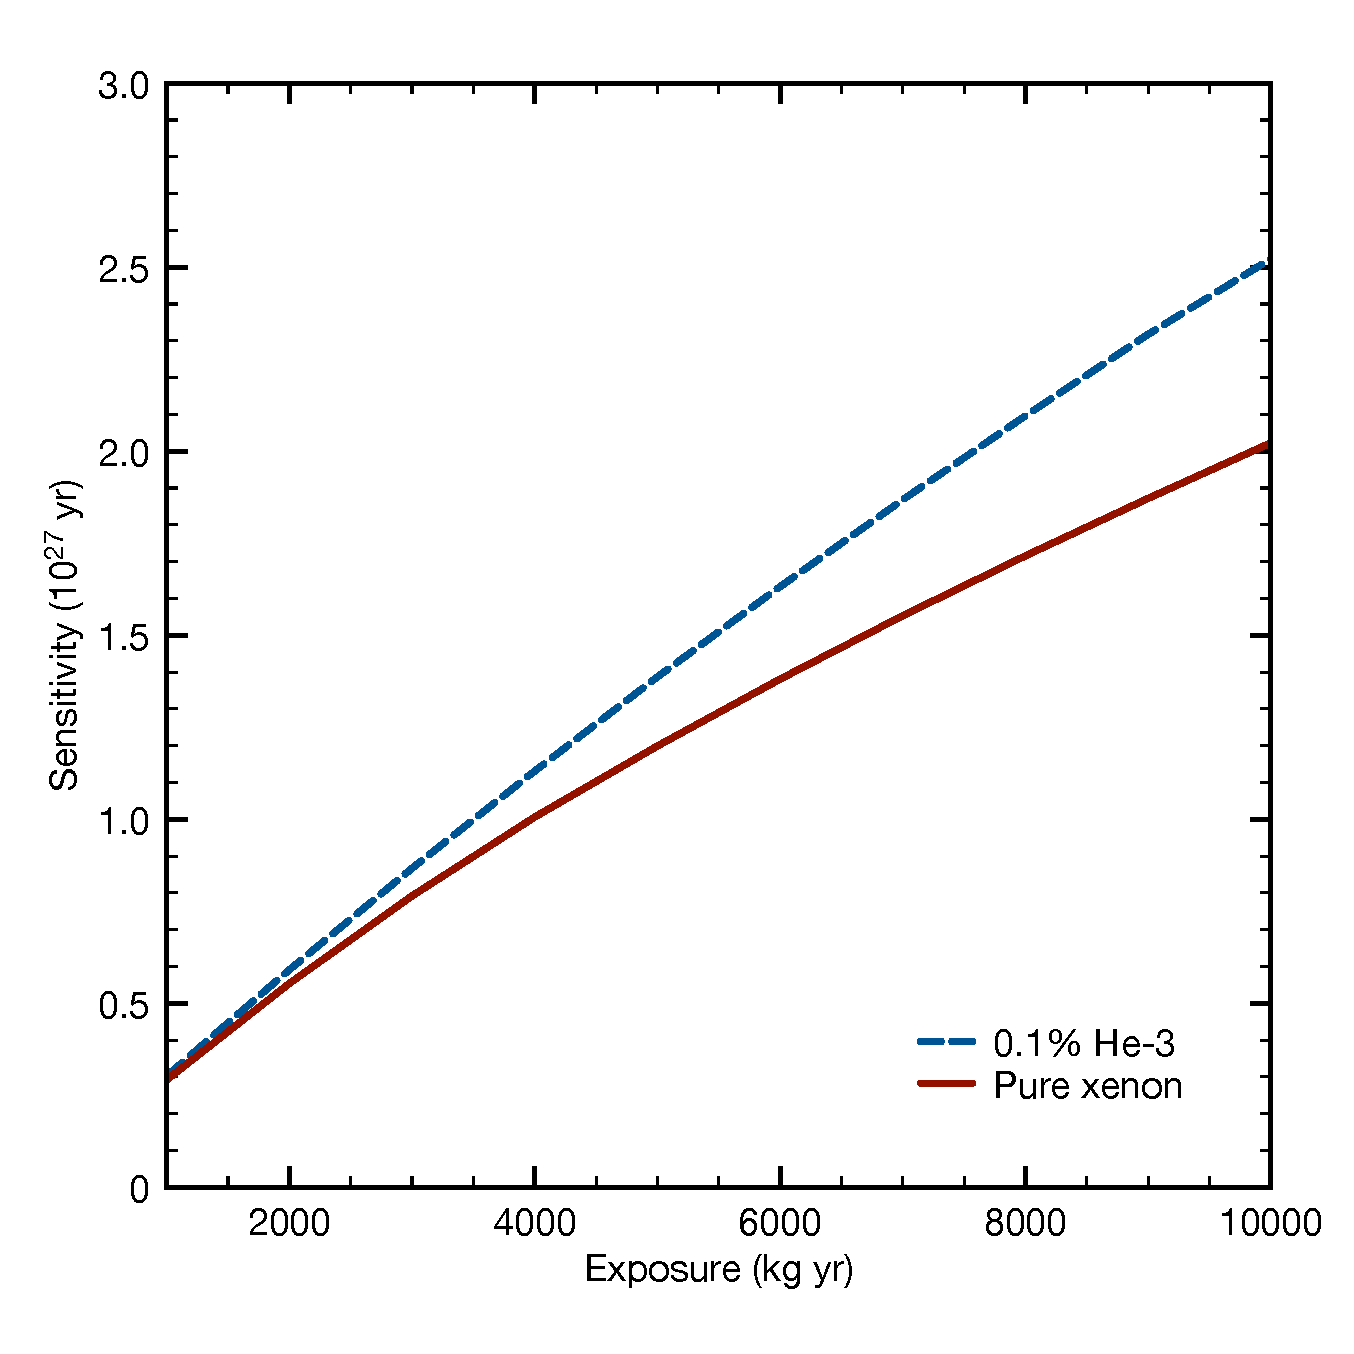
\includegraphics[width=0.85\textwidth]{img/sensitivity_nexthd_lsc.pdf}
%\caption{Projected sensitivity (90\% CL) to the \Xe{136} \bbonu\ half-life for a NEXT ton-scale experiment located at LSC. \label{fig:Sensitivity}}
%\end{figure}

\subsection{The \HDEMO\ prototype}

\begin{figure}
  \begin{center}
    %\includegraphics[width=0.31\textwidth]{img/Fiber13D.png}
    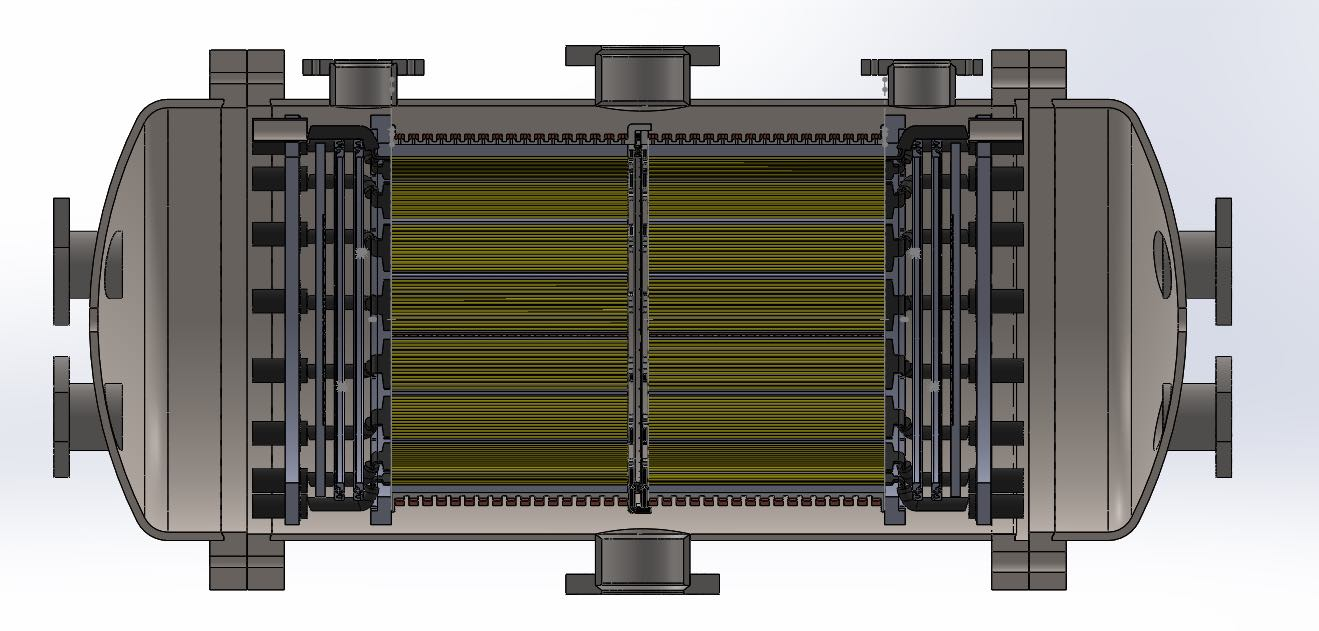
\includegraphics[width=0.51\textwidth]{img2/nhd_vessel.jpg}
    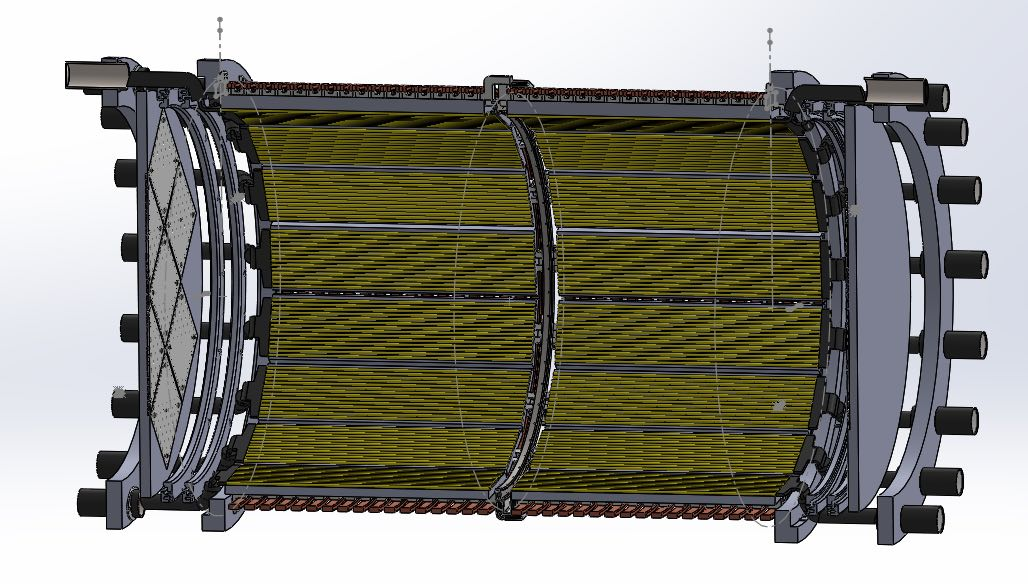
\includegraphics[width=0.45\textwidth]{img2/nhd_view.jpg}
    \caption{Conceptual design of the \HDEMO. The left panel shows a lateral view including the vessel. Notice the symmetric structure and the ports for
    the high voltage feedthroughs. In this design, shown in more detail in the right panel, the fibers are read out by PMTs disposed as a ring around the silicon planes.} 
    \label{fig.hdemo}
  \end{center}
\end{figure}


\indent


The R\&D towards \NHD\ requires the construction, commissioning and operation of a mid-size demonstrator that we call \HDEMO. The apparatus, shown in figure \ref{fig.nhd}, will permit addressing several key questions. Specifically:

\indent


\begin{itemize}[noitemsep,topsep=0pt,parsep=0pt,partopsep=0pt]
\item Demonstrate the expected light yield and energy resolution of the BDF (we project 0.5\%--0.7\% FWHM). Decide whether the fibres will be readout using PMTs (as shown in figure \ref{fig.hdemo}) or by SiPMs. 
\item Demonstrate the improvement of the topological signature using DSPs (pitch of 7 mm) and Xe-He mixtures. Find the best compromise between pitch, diffusion and cost. 
\item Assess the potential of new materials, in particular titanium vs low radioactivity steel alloys, for the pressure vessel and the grids. 
\item Gain experience with the construction and integration of a symmetric TPC (all previous NEXT incarnations have been asymmetric). 
\item Test the new electronics for the BFD and DSP.
\item Test the new DAQ for \NHD.  
\item Test the overall system integration. 
\end{itemize}

\indent


The detector will have a diameter of \HDD and a length of \HDL, divided in two identical halves. The central cathode will be at a high voltage of \HDHV, while the two anodes will be at ground. The vessel will stand a pressure in excess of 20 bars. The operational pressure will be the same than \Next\ (and foreseen for \NHD), \eg, 15 bars. The xenon mass at that pressure will be \HDM. 

\indent


The three main systems of \HDEMO are a prototype of the BFD (pBFD), a prototype of the DSPs (pDSP) and a prototype of the TPC (pTPC). The detector will be hosted in a pressure vessel (PV) made of steel or titanium, and protected by an external lead shield, but no inner copper shield is necessary (the operation of the detector, with radioactive sources, does not require ultra-low background). The operation of \HDEMO\ requires a fully equipped laboratory and a state-of-the-art gas system, all of which will be provided by the laboratory hosting the apparatus (DIPC). 

%%%%%%%%%%